\section{Introduction}

Au commencement du projet, un ensemble majeur de fonctionnalités - notamment la synchronisation, la résolution de conflits à l'aide de types de données répliqués sans conflit (CRDT), la gestion des clés cryptographiques et l'implémentation réseau - devait être réalisé par une entreprise externe. Cependant, pour diverses raisons, ce partenariat n'a pas abouti. Ceci a conduit à une réorientation majeure du projet : l'ensemble de ces fonctionnalités a dû être conçu et mis en œuvre en interne.

C'est ainsi que le Decentralized Document Network (DDnet) a vu le jour. DDnet est un système de gestion de documents décentralisé axé sur le principe du "Local-First". Il permet de partager et de synchroniser des documents en temps réel entre plusieurs utilisateurs, le tout de manière sécurisée et chiffrée de bout en bout.

\section{Authentification et Gestion des Clés}

Le système conçu lors de ce projet identifie chaque utilisateur par sa clé publique. Les clés sont générées grâce à un système mnémonique inspiré de BIP39\footnote{\url{https://github.com/bitcoin/bips/blob/master/bip-0039.mediawiki}}, une norme facilitant la génération d'une clé privée à partir d'une phrase secrète, ce qui favorise la sauvegarde et la restauration des clés.

La réimplémentation du module npm \textit{bip39} a été nécessaire en raison de son incompatibilité avec les navigateurs, étant initialement conçu pour Node.js. Les fonctions et objets spécifiques à Node.js ont été substitués par leurs équivalents navigateur pour assurer la compatibilité. La taille du package a été significativement réduite, de 331 Ko à 57 Ko, grâce à cette réimplémentation, la rendant ainsi plus appropriée pour une utilisation navigateur. Le module réimplémenté est disponible sur npm sous le nom \textit{@describble/srp} (Secret Recovery Phrase)\footnote{\url{https://www.npmjs.com/package/@describble/srp}}.

Conformément au paradigme "Local-First", les clés privées sont stockées localement dans le navigateur de l'utilisateur. Cependant, le stockage en clair de ces clés serait problématique pour des raisons de sécurité. Par conséquent, les clés privées sont chiffrées à l'aide d'un mot de passe utilisateur. Ce mot de passe est d'abord dérivé via la fonction de dérivation PBKDF2\footnote{\url{https://en.wikipedia.org/wiki/PBKDF2}} avant d'être utilisé pour le chiffrement. Un sel aléatoire et un nombre d'itérations fixé à 10000 sont utilisés pour renforcer la sécurité de la dérivation. La clé dérivée est ensuite utilisée avec l'algorithme AES-GCM pour chiffrer la clé privée. Il convient de noter que le mot de passe n'est jamais stocké en clair ni transmis sur le réseau, il est seulement utilisé pour la dérivation de la clé de chiffrement.

J'ai également anticipé que plusieurs utilisateurs pourraient partager le même navigateur. Ainsi, pour préserver la confidentialité des données de chaque utilisateur, il est nécessaire de chiffrer les données spécifiques à chaque utilisateur. Cette mesure garantit que chaque utilisateur peut utiliser le même navigateur sans avoir accès aux données des autres.

La gestion des sessions est une partie délicate et complexe du système. Pour pouvoir signer ou chiffrer les données, le système doit avoir accès à la clé privée. Cependant, stocker cette clé en clair dans le navigateur serait inacceptable pour des raisons de sécurité. C'est pourquoi la clé privée en clair est uniquement stockée en mémoire. Cependant, la mémoire est effacée lors du rafraîchissement de la page. Pour pallier ce problème, j'ai décidé d'utiliser un Service Worker\footnote{\url{https://developer.mozilla.org/en-US/docs/Web/API/Service_Worker_API}}, dont le cycle de vie est indépendant de la page. Ainsi, la clé privée peut être stockée dans le worker et utilisée par la page. Toutefois, cette solution présente certaines limites, le cycle de vie d'un Service Worker étant indéterminé : il peut être détruit à tout moment par le navigateur, sans moyen de le prévoir.

\section{Connectivité et Serveur de Signalisation}

La capacité de synchroniser et partager des documents en temps réel constitue une fonctionnalité essentielle du système élaboré dans le cadre de ce projet. Cependant, pour respecter l'impératif de décentralisation, il est impossible de s'appuyer sur un serveur centralisé. WebRTC, un standard du W3C facilitant la communication en temps réel entre navigateurs, a donc été sélectionné pour établir une connexion pair à pair.

\subsection{Signalisation et Établissement de Connexion}

Néanmoins, pour que deux navigateurs puissent communiquer via WebRTC, ils doivent pouvoir se localiser sur le réseau. Cela nécessite l'intervention d'un serveur de signalisation, dont le rôle est de permettre aux navigateurs d'échanger les informations nécessaires pour établir une connexion directe. Une fois cette connexion établie, le serveur de signalisation n'intervient plus. Bien que des bibliothèques comme PeerJS\footnote{\url{https://peerjs.com/}} proposent un serveur de signalisation, elles ne sont pas compatibles avec le système d'authentification développé pour ce système. De ce fait, un serveur de signalisation personnalisé a été implémenté.

Le serveur de signalisation est un serveur Web qui recourt au protocole WebSocket, un protocole de communication bidirectionnel, pour instaurer une connexion persistante entre le client et le serveur. Pour l'implémentation du serveur de signalisation, Node.js a été choisi, en utilisant la bibliothèque ws\footnote{\url{https://www.npmjs.com/package/ws}} pour le protocole WebSocket. Bien que centralisé, le serveur de signalisation n'est pas un point de faiblesse du système. En effet, il ne traite pas de données sensibles et se contente de faciliter l'établissement d'une connexion directe entre deux clients. De plus, le serveur de signalisation est open-source et peut être auto-hébergé par les utilisateurs.

\subsection{Authentification par Serveur}

Le serveur de signalisation possède un module d'authentification, composé de trois classes distinctes : la classe Authenticator de base, la classe ServerAuthenticator, et la classe ClientAuthenticator. Ces classes sont conçues pour vérifier l'authenticité des connexions grâce à un mécanisme de poignée de main basé sur un défi-réponse cryptographique.

\subsubsection{Mécanisme de Défi-Réponse}

Le mécanisme de défi-réponse est une méthode pour prouver une identité en démontrant la connaissance d'un secret sans le révéler. Ici, un défi aléatoire est généré par le serveur et envoyé au client. Le client génère ensuite une réponse au défi en utilisant sa clé privée, qui peut être vérifiée avec la clé publique du client connue du serveur. Cela garantit l'identité du client, car seul le détenteur valide de la clé privée peut générer une réponse correcte.

Le processus d'authentification suit les étapes suivantes :

\begin{enumerate}
\item Le serveur envoie un défi aléatoire au client.
\item Le client reçoit le défi et crée une signature de réponse en utilisant sa clé privée.
\item Le client renvoie la réponse signée au serveur.
\item Le serveur vérifie la réponse en utilisant la clé publique du client.
\item Si la vérification est réussie, le serveur reconnait le client comme authentifié. Sinon, il ferme la connexion.
\end{enumerate}

\begin{figure}[H]
  \begin{center}
      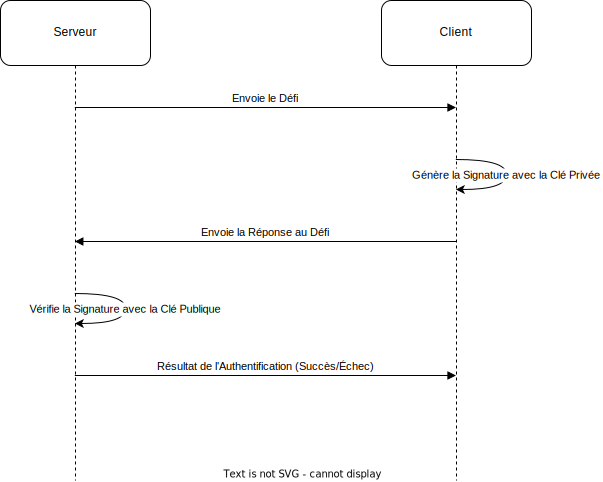
\includegraphics[width=0.75\textwidth]{\assetsdir/diagram-ddnet-auth.svg} % half of the text width
  \end{center}
  \caption[Mécanisme de Défi-Réponse]{Le diagramme représente le processus du mécanisme de défi-réponse utilisé pour l'authentification.}
\end{figure}

\subsection{Routage des Messages}

Le serveur de signalisation est responsable du routage des messages entre les clients. Pour ce faire, il maintient un registre des clients et de leurs connexions. Chaque client peut avoir plusieurs connexions, et chaque connexion est identifiée de manière unique par un ID de client généré de manière aléatoire. Ceci, associé à la clé publique du client, nous permet d'envoyer un message à tous les clients, à toutes les connexions d'un client spécifique, ou à une connexion spécifique.

\begin{figure}[H]
  \begin{center}
    \includegraphics[width=0.75\textwidth]{\assetsdir/diagram-ddnet-registry.svg}
  \end{center}
  \caption[Registre et Connexions]{Illustration du registre du serveur contenant les clés publiques des clients et leurs connexions associées.}
\end{figure}

\subsection{Structure du Message}

La structure d'un message est conçue avec la flexibilité et la sécurité à l'esprit :

\begin{listing}[H]
  \begin{minted}[breaklines]{typescript}
  type Message<TData> = {
      from: {
        publicKey: Uint8Array;  // sender's public key
        clientId: Uint8Array;   // sender's clientId
      };
      to?: {
        publicKey: Uint8Array;  // recipient's public key
        clientId?: Uint8Array;  // recipient's clientId (optional)
      };
      data: TData;              // payload data of the message
  };
  \end{minted}
  \caption{Type Typescript de la structure d'un Message} 
  \end{listing}

Le champ from identifie l'expéditeur du message.
Le champ to est facultatif et identifie le destinataire du message. Ce champ est nécessaire lorsque le message est privé et destiné à un utilisateur spécifique. Si le champ to est omis, le message est considéré comme public et peut être lu par n'importe quel utilisateur du réseau.
Le champ data contient les véritables données de la charge utile du message.

\subsection{Chiffrement des Messages}

Le système chiffre automatiquement les messages si la clé publique du destinataire est spécifiée. Il implémente un protocole de transmission sécurisé, qui utilise la cryptographie pour maintenir la confidentialité et l'intégrité des messages. Les opérations cryptographiques spécifiques utilisées incluent :

\begin{itemize}
\item \textbf{Diffie-Hellman sur courbes elliptiques (ECDH)} : Un protocole d'échange de clés qui permet à deux parties d'établir un secret partagé sur un canal non sécurisé. Ce secret partagé est généré en utilisant la clé privée de l'expéditeur et la clé publique du destinataire.
\item \textbf{Fonction de dérivation de clés basée sur un mot de passe 2 (PBKDF2)} : Une fonction de dérivation de clés utilisée pour dériver une clé AES à partir du secret partagé obtenu lors de l'échange ECDH. Elle ajoute un sel pour la randomisation, offrant une résistance contre les attaques par dictionnaire.
\item \textbf{Advanced Encryption Standard - Galois/Counter Mode (AES-GCM)} : Cet algorithme de chiffrement symétrique utilise la clé AES dérivée pour chiffrer le message, garantissant ainsi que seul le destinataire prévu peut le déchiffrer et le lire. L'AES-GCM assure à la fois la confidentialité et l'intégrité des données.
\item \textbf{Algorithme de signature numérique sur courbes elliptiques (ECDSA) avec la courbe secp256k1} : Après que le message a été chiffré, il est signé en utilisant la clé privée de l'expéditeur. La signature permet de vérifier l'authenticité de l'expéditeur et confirme que le message n'a pas été altéré pendant la transmission.
\end{itemize}

Ce protocole assure une communication sécurisée et confidentielle, où seuls les destinataires prévus peuvent déchiffrer et lire le message. Il vérifie également l'authenticité de l'expéditeur et garantit l'intégrité du message.

\subsection{Transmission des Messages}

Les messages dans ce système peuvent être transmis de trois manières différentes en fonction du destinataire cible :

\begin{itemize}
\item \textbf{Broadcast} : Un message est diffusé à tous les utilisateurs du réseau. C'est la méthode de transmission par défaut lorsque le champ `to` est omis.
\item \textbf{Multicast} : Un message est envoyé à un utilisateur spécifique du réseau. C'est la méthode de transmission par défaut lorsque le champ `to` est spécifié, mais que le champ `clientId` est omis.
\item \textbf{Unicast} : Un message est envoyé à une session spécifique d'un utilisateur dans le réseau. C'est la méthode de transmission par défaut lorsque le champ `to` est spécifié et que le champ `clientId` est spécifié.
\end{itemize}

La sécurité est une préoccupation majeure dans la transmission des messages dans ce système. Chaque message est signé numériquement par l'expéditeur, ce qui permet au serveur de vérifier son intégrité à la réception. Si le serveur détecte que le message a été altéré pendant la transmission, il le supprime immédiatement et arrête sa propagation.

La signature numérique garantit non seulement que le message provient bien de l'expéditeur déclaré, mais elle permet également de détecter tout changement ou corruption du contenu du message. Cela est crucial pour maintenir la confiance et la fiabilité du système de communication.

Voici un diagramme représentant la logique de routage :

\begin{figure}[H]
  \begin{center}
      \includegraphics[width=0.75\textwidth]{\assetsdir/diagram-ddnet-routing.svg}
  \end{center}
  \caption[Logique de Routage des Messages]{Schéma illustrant la logique de routage des messages dans le système.}
\end{figure}


\section{Gestionnaire de documents}
\subsection{Structure des documents}
#TODO : Structure des documents, Headers, etc.
\subsection{Synchronisation}
#TODO : Utilisation de Automerge, etc.
\subsection{Sécurité des documents}
#TODO : Chiffrement des documents, autorisations, etc.
\subsection{Stockage des documents}
#TODO : Stockage des documents, IndexDB, etc.

\section{Module de présence}
#TODO : Messages éphémères par document.
